% =============================================================================
% COPYRIGHT AND DISCLAIMER
% =============================================================================
% This file is provided as a convenience template for competition participants.
% By using it, you accept full responsibility for compliance with all applicable
% copyright, licensing, and usage rules of the Association for Computing
% Machinery (ACM) and of any LaTeX packages you load (including, without
% limitation, the "acmart" document class and related ACM materials).
%
% Consult ACM's official publication, template, and copyright policies before
% using this setup for any purpose other than this competition. Do not assume
% that this template may be reused, redistributed, or submitted elsewhere
% without independently verifying ACM's current rules.
%
% Use of the "acmart" class, the "sigconf" option, or ACM-style formatting in
% this template does NOT mean that this report, this competition, its organizers,
% or any resulting PDF is sponsored, endorsed, affiliated with, or published by
% ACM. ACM trademarks and branding remain the property of ACM.
%
% Template packages live in preamble.tex.
% Citations live in main.bib. Edit this file with your paper content.
% =============================================================================

\documentclass[sigconf]{acmart}
% =============================================================================
% Template setup — participants normally do not edit this file.
% Author content belongs in main.tex; citations belong in main.bib.
% \documentclass lives in main.tex so Overleaf does not treat this file as root.
% =============================================================================

% --- Competition / non-ACM-submission friendly rights metadata -------------
\setcopyright{none}
\settopmatter{printacmref=false}
\acmConference[Kaggle Competition]{Filament Segmentation Challenge}{2026}{\href{https://www.kaggle.com/competitions/filament-segmentation-2026}{kaggle.com/competitions/filament-segmentation-2026}}
\acmBooktitle{Competition Report}
\acmDOI{}
\acmISBN{}

% --- Author guidance text --------------------------------------------------
% \guide{...} is gray italic while \guideStyletrue; omitted from the PDF if false.
% Flip the switch in main.tex after % =============================================================================
% Template setup — participants normally do not edit this file.
% Author content belongs in main.tex; citations belong in main.bib.
% \documentclass lives in main.tex so Overleaf does not treat this file as root.
% =============================================================================

% --- Competition / non-ACM-submission friendly rights metadata -------------
\setcopyright{none}
\settopmatter{printacmref=false}
\acmConference[Kaggle Competition]{Filament Segmentation Challenge}{2026}{\href{https://www.kaggle.com/competitions/filament-segmentation-2026}{kaggle.com/competitions/filament-segmentation-2026}}
\acmBooktitle{Competition Report}
\acmDOI{}
\acmISBN{}

% --- Author guidance text --------------------------------------------------
% \guide{...} is gray italic while \guideStyletrue; omitted from the PDF if false.
% Flip the switch in main.tex after % =============================================================================
% Template setup — participants normally do not edit this file.
% Author content belongs in main.tex; citations belong in main.bib.
% \documentclass lives in main.tex so Overleaf does not treat this file as root.
% =============================================================================

% --- Competition / non-ACM-submission friendly rights metadata -------------
\setcopyright{none}
\settopmatter{printacmref=false}
\acmConference[Kaggle Competition]{Filament Segmentation Challenge}{2026}{\href{https://www.kaggle.com/competitions/filament-segmentation-2026}{kaggle.com/competitions/filament-segmentation-2026}}
\acmBooktitle{Competition Report}
\acmDOI{}
\acmISBN{}

% --- Author guidance text --------------------------------------------------
% \guide{...} is gray italic while \guideStyletrue; omitted from the PDF if false.
% Flip the switch in main.tex after \input{preamble}.
%
% Do not use \guide{...} for \email{...}.
\usepackage{xcolor}
\newif\ifguideStyle
\guideStyletrue
\newcommand{\guide}[1]{%
  \ifguideStyle
    {\color{gray!65}\itshape #1}%
  \fi
}

% --- Math ------------------------------------------------------------------
% Do NOT load amssymb (or amsfonts): acmart already loads newtxmath, which
% defines the same symbols (e.g. \Bbbk) and causes a conflict on Overleaf.
% amsmath is already provided by acmart; mathtools extends it.
\usepackage{mathtools}

% --- Figures ---------------------------------------------------------------
% graphicx is already loaded by acmart
\usepackage{subcaption}

% --- Tables ----------------------------------------------------------------
% booktabs is already loaded by acmart
\usepackage{tabularx}
\usepackage{multirow}

% --- Bibliography style is set in main.tex (ACM-Reference-Format) ----------
.
%
% Do not use \guide{...} for \email{...}.
\usepackage{xcolor}
\newif\ifguideStyle
\guideStyletrue
\newcommand{\guide}[1]{%
  \ifguideStyle
    {\color{gray!65}\itshape #1}%
  \fi
}

% --- Math ------------------------------------------------------------------
% Do NOT load amssymb (or amsfonts): acmart already loads newtxmath, which
% defines the same symbols (e.g. \Bbbk) and causes a conflict on Overleaf.
% amsmath is already provided by acmart; mathtools extends it.
\usepackage{mathtools}

% --- Figures ---------------------------------------------------------------
% graphicx is already loaded by acmart
\usepackage{subcaption}

% --- Tables ----------------------------------------------------------------
% booktabs is already loaded by acmart
\usepackage{tabularx}
\usepackage{multirow}

% --- Bibliography style is set in main.tex (ACM-Reference-Format) ----------
.
%
% Do not use \guide{...} for \email{...}.
\usepackage{xcolor}
\newif\ifguideStyle
\guideStyletrue
\newcommand{\guide}[1]{%
  \ifguideStyle
    {\color{gray!65}\itshape #1}%
  \fi
}

% --- Math ------------------------------------------------------------------
% Do NOT load amssymb (or amsfonts): acmart already loads newtxmath, which
% defines the same symbols (e.g. \Bbbk) and causes a conflict on Overleaf.
% amsmath is already provided by acmart; mathtools extends it.
\usepackage{mathtools}

% --- Figures ---------------------------------------------------------------
% graphicx is already loaded by acmart
\usepackage{subcaption}

% --- Tables ----------------------------------------------------------------
% booktabs is already loaded by acmart
\usepackage{tabularx}
\usepackage{multirow}

% --- Bibliography style is set in main.tex (ACM-Reference-Format) ----------


% Guide styling: \guideStyletrue = show gray italic hints; \guideStylefalse = omit them
\guideStylefalse
% \guideStyletrue

\begin{document}

\title{Detector-Guided Native-Resolution Refinement for Solar Filament Instance Segmentation}
\subtitle{A Solution to the Solar Filament Segmentation Challenge 2026} % DO NOT CHANGE


\author{Kuan Ta Wu}
\affiliation{%
  \institution{Max Well Apex LLC}
  \city{New York}
  \country{USA}
}
\email{YOUR-EMAIL-HERE}   % TODO: replace with the submitting author's email before filing

% \author{\guide{Second Author}}
% \affiliation{%
%   \institution{\guide{Your Institution}}  % <- Optional (remove if you are not currently affiliated with any institute)
%   \city{\guide{City}}
%   \country{\guide{Country}}
% }
% \email{second.author@example.com}  % <- Replace with your own email

\begin{abstract}
    This report describes our solution to the Solar Filament Segmentation Challenge~2026, a Kaggle competition on automatic segmentation of solar filaments in GONG H-$\alpha$ observations. We use a two-stage instance pipeline: a COCO-pretrained Mask R-CNN (ResNet50 FPN v2) localizes filaments at $1024^2$, then a ResNet18 U-Net refiner re-segments each detection from a native-resolution $256^2$ crop, with topology-safe four-flip test-time augmentation. All selection uses date-disjoint splits (582 fit / 63 tuning / 62 holdout photographs; annotator views never split across partitions). At native $2048^2$ resolution, pooled over all holdout annotator views, the detector alone reaches Panoptic Quality (PQ) 0.3421 and the full pipeline 0.4209, above our strongest semantic-segmentation baselines (0.3927--0.4068 on a $1024^2$ grid). Every candidate in the development ladder is frozen, hash-verified, and reproducible from the public repository.
    % PUBLIC-SCORE: add the pipeline public score + submission ref here after scoring.
\end{abstract}

\maketitle

% ==================================== %
%              INTRODUCTION            %
% ==================================== %
\section{Introduction}
    This report goes over the details of our submitted solution to the Solar Filament Segmentation Challenge~2026 \cite{filament-segmentation-2026}. The challenge, launched on July~10,~2026, is organized by the Earth-Space AI Research (ESAIR) Lab\footnote{\href{https://www.esairlab.com/home}{www.esairlab.com/}}. This challenge utilizes the MAGFiLO dataset for evaluation of the segmentation algorithms \cite{ahmadzadeh2024dataset}. The task is instance segmentation scored by Panoptic Quality~\cite{kirillov2019panoptic}: each filament needs its own accurate mask, so merged, fragmented, missed, and spurious objects are all penalized.

    Our early entries were semantic U-Nets whose connected components defined instances. They improved steadily (public scores 0.20 $\rightarrow$ 0.26 $\rightarrow$ 0.30) but plateaued: an error decomposition of the best semantic model showed partial-overlap masks and spurious components dominating over merge/split errors, and three later candidates with holdout PQ 0.395--0.407 all scored 0.29 in public. We therefore switched model family for the final candidate: object detection supplies instance identity and recall, and a per-instance refiner operating at native resolution supplies boundary accuracy. This report documents that pipeline, its selection protocol, and its limitations; local scores are never presented as official leaderboard results.

% ==================================== %
%              METHODOLOGY             %
% ==================================== %
\section{Methodology}\label{sec:methodology}

\begin{figure*}[t]
\centering
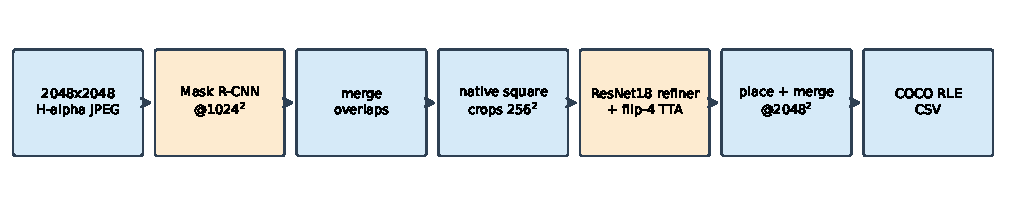
\includegraphics[width=0.92\textwidth]{fig_pipeline.pdf}
\Description{Flow diagram: full-disk image, Mask R-CNN detection, overlap merge, native crops, ResNet18 refiner with flip TTA, placement at native resolution, and COCO RLE output.}
\caption{End-to-end pipeline. Detection runs on the $1024^2$ frame; all boundary decisions after detection are made on native-resolution crops and placed back at $2048^2$.}
\label{fig:pipeline}
\end{figure*}

\subsection{Data and sampling strategy}
The competition release contains 707 labeled physical photographs (1,154 image--annotator views; 8,199 polygon instances) and 180 unlabeled test photographs, all $2048^2$ GONG H-$\alpha$ JPEGs~\cite{ahmadzadeh2024dataset,filament-segmentation-2026}. We partition photographs by observation \emph{date} into 582 fit, 63 tuning, and 62 holdout images; every annotator view of a photograph stays in the same partition, so near-duplicate images cannot leak across splits. Detector and refiner training consume one selected annotator view per photograph (the view with the most annotated instances, then most area), because instance training needs one consistent target set per image. Evaluation instead pools predictions against \emph{every} annotator view, so annotator disagreement is priced into all reported numbers. No labels beyond the competition training set are used; in particular we do not train on the larger public MAGFiLO archive, whose additional labels could overlap organizer-held data. Test images are used for inference only.

\subsection{Stage 1: Mask R-CNN detector}
The detector is Mask R-CNN with a ResNet50 FPN v2 backbone initialized from public COCO weights~\cite{he2017maskrcnn}, with both predictors replaced for two classes (background, filament). Anchor sizes (16--256) and aspect ratios (0.5/1/2) are set for thin elongated objects, and the mask RoI pooler outputs $28\times28$ to retain strand detail. Inputs are grayscale frames area-downsampled to $1024^2$ and repeated to three channels. Augmentation is random quarter-turns, horizontal flips, and photometric gamma/contrast/blur/noise applied on the solar disk only. Training uses SGD (learning rate $5\times10^{-3}$, momentum 0.9, weight decay $10^{-4}$, batch 2, mixed precision, ten epochs, learning-rate drops at 70\% and 90\%); the checkpoint is selected by tuning-split PQ of the merged detector masks (best at epoch 6). The detector's role is recall with object identity; its coarse mask head is not trusted for final boundaries.

\subsection{Stage 2: native-resolution crop refiner}
For every ground-truth filament we extract a square crop from the original $2048^2$ image (side $1.8\times$ the instance bounding box, minimum 96\,px), resized to $256^2$ together with its binary mask. A U-Net with an ImageNet-pretrained ResNet18 encoder~\cite{he2016resnet} is trained on these crops with an equally weighted BCE + soft-Dice loss (AdamW, $3\times10^{-4}$, batch 16, eight epochs, cosine schedule), reaching tuning-crop Dice 0.8149. Because crops come from native pixels, thin barbs that disappear in whole-image downsampling remain visible to the refiner.

\subsection{Inference, TTA, and assembly}
Detections with score $\ge 0.70$ and mask probability $\ge 0.50$ are kept and positively overlapping masks are unioned into refinement groups. Each group is upscaled to $2048^2$, cropped with the same square-bounds rule, and refined. The refiner runs on the identity, horizontal, vertical, and combined flips of each crop; the de-flipped average is accepted only when it preserves the single-view topology (area ratio within $[0.60, 1.70]$, component count grows by at most one, and Dice against the single-view mask at least 0.62 for non-trivial masks), otherwise the single-view probability is kept. The chosen probability is resized back to the crop bounds, thresholded at 0.60, and placed at native resolution; an empty refinement falls back to the detector mask, so refinement can redraw but never silently delete a detection. Positively overlapping refined masks are merged, and every remaining object is serialized as compressed COCO RLE counts in column-major order~\cite{coco}. The three operating thresholds were selected by a nine-point grid on the tuning split and frozen before holdout confirmation; Figure~\ref{fig:qualitative} shows one held-out example.

\begin{figure*}[t]
\centering
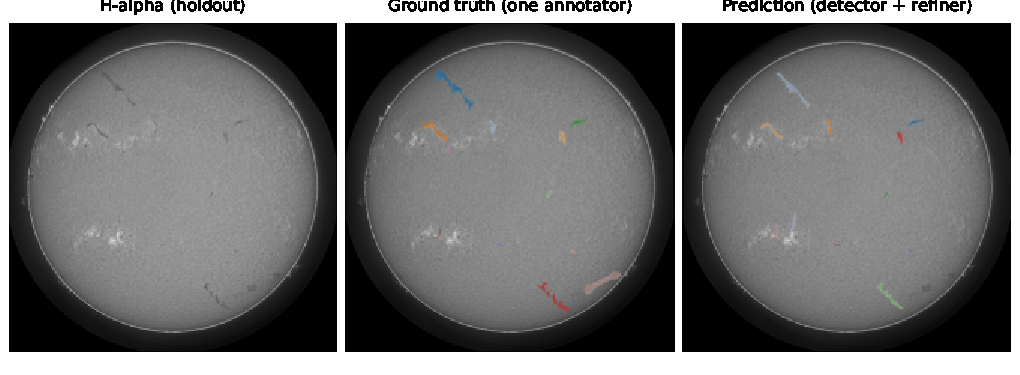
\includegraphics[width=0.95\textwidth]{fig_qualitative.pdf}
\Description{Three panels: a held-out H-alpha full-disk image, colored ground-truth filament instances from one annotator, and colored predicted instances.}
\caption{Held-out observation 20110601063134Lh: H-$\alpha$ image (left), one annotator's ground truth (center), and the pipeline prediction (right). Colors are per-panel instance identifiers and are not matched across panels. The bottom-right pair illustrates a remaining merge error.}
\label{fig:qualitative}
\end{figure*}

% ==================================== %
%              EVALUATION              %
% ==================================== %
\section{Evaluation}\label{sec:evaluation}
For every annotator view we match predicted and ground-truth instances at $\operatorname{IoU}>0.5$ and pool counts over views and photographs:
\begin{equation}
\mathrm{PQ}=\frac{\sum_{(y,\hat y)\in TP}\mathrm{IoU}(y,\hat y)}{|TP|+\frac12|FP|+\frac12|FN|}.
\end{equation}
Semantic baselines are scored on the $1024^2$ grid they predict on; the two-stage pipeline is scored at native $2048^2$. Both use the identical date-disjoint holdout photographs and pooled all-view protocol, so rows are comparable as candidate rankings, with the grid noted per row. We report single-split point estimates without error bars: the holdout informed ranking among a handful of frozen candidates, and differences below roughly 0.01 PQ already failed to reproduce on the public split, so we treat them as ties rather than improvements.

\begin{table}[t]
\caption{Development ladder on the 62-photograph holdout (tune-selected configurations) and the resulting public leaderboard (LB) scores. Semantic rows are scored on a $1024^2$ grid; pipeline rows at native $2048^2$.}
\label{tab:ladder}
\centering
\begin{tabular}{lrr}
\toprule
Candidate & Holdout PQ & Public LB\\
\midrule
Compact U-Net (shipped) & --- & 0.20\\
DeepUNet base16 & 0.3644 & 0.26\\
DeepUNet base24 & 0.3927 & 0.30\\
DeepUNet base32 & 0.3989 & 0.29\\
SMP U-Net ResNet34 & 0.3951 & ---\\
Long base32 (crop 640) & 0.4068 & 0.29\\
Detector only (native) & 0.3421 & ---\\
\textbf{Detector + refiner (native)} & \textbf{0.4209} & \textbf{0.34}\\
\bottomrule
\end{tabular}
\end{table}

\begin{figure}[t]
\centering
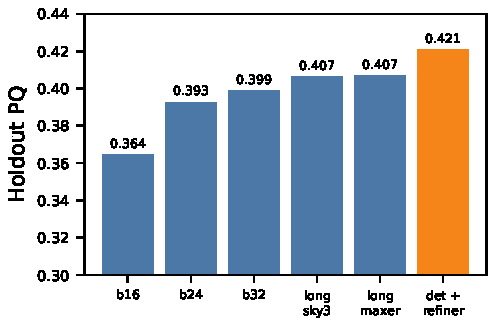
\includegraphics[width=\columnwidth]{holdout_ladder.pdf}
\Description{Bar chart of tune-selected holdout PQ for six candidates; the native-resolution detector-plus-refiner bar is the highest.}
\caption{Tune-selected holdout PQ across the development ladder. Semantic candidates are scored on their $1024^2$ grid; the two-stage pipeline is scored at native $2048^2$.}
\label{fig:ladder}
\end{figure}

Three observations drive the final design. First, the refiner is worth +0.079 PQ over the detector alone (0.3421 to 0.4197 at the initial operating point): detector masks localize objects, but only native-resolution crops draw boundaries accurate enough for the IoU 0.5 gate. Second, an error decomposition of the best semantic model (union Dice 0.691) showed partial-overlap masks and spurious components dominating over merge/split errors, which is why we invested in per-instance refinement and conservative detector thresholds rather than post-hoc splitting heuristics. Third, holdout gains of a few thousandths did not transfer to the public split (three candidates with holdout 0.395--0.407 all scored 0.29), so we select by holdout but report public scores without extrapolating them.

An all-data final-fit variant (fit+tune, fixed epochs 6/8) reached holdout PQ 0.4123 and was rejected in favor of the tune-selected checkpoints above; probability-averaged ensembles of the semantic models (0.3844--0.4060) were likewise evaluated and not selected. The submitted candidate contains 1,585 instances across the 180 test images (three images empty), with SHA-256 \texttt{e1e95bf387\ldots} recorded in the repository audit file.
On the public leaderboard this candidate scored 0.34 (submission ref.\ 58254552), the best of our six submissions; the private score is not yet known.

\textbf{Reproducibility and compliance.} The release contains the training and inference code, both checkpoints (the detector exceeds GitHub's 100\,MB file limit and is distributed as a release asset with its SHA-256 in the README), all evaluation JSONs, and the exact candidate CSV with its audit file. Every submitted RLE row is verified to sum to $2048^2$ pixels with unique per-image identifiers before upload. Inference consumes only the official test JPEGs. Pretrained weights are the public COCO Mask R-CNN and ImageNet ResNet18 weights~\cite{he2017maskrcnn,he2016resnet}; no external labels, no full-MAGFiLO labels beyond the competition set, and no test-derived statistics are used anywhere in training or threshold selection. AI assistance was used to write and verify code and to draft this report; technical responsibility remains with the submitting participant.

\textbf{Strengths, weaknesses, and improvements.} The pipeline's strength is instance identity from detection plus native-resolution boundaries from refinement, which together remove the two largest semantic-model error classes. Its weaknesses are equally specific: detection still runs at $1024^2$, so the faintest strands can be missed before refinement; positively overlapping refined masks are merged, which can re-join crowded neighbors (visible at bottom-right in Figure~\ref{fig:qualitative}); and inter-annotator disagreement imposes a ceiling that no threshold choice removes. The most direct follow-ups are a conservative detector-seed split for crowded groups, annotator-consensus modeling validated prospectively, and higher-resolution detection once compute allows. Until then, the submitted configuration is the one frozen by the tuning split, not the best-looking row in hindsight.

% ==================================== %
%            ACKNOWLEDGMENT            %
% ==================================== %
\section{Acknowledgment}\label{sec:acknowledgment}
    % Do not change
    The organization of the Filament Segmentation Challenge 2026 is partially supported by the U.S. National Science Foundation (NSF) under Grant No. 2209912 and 2433781, directorate for Computer and Information Science and Engineering (CSE), and Office of Advanced Cyberinfrastructure (OAC), and Grant No. 2511630, AST Division Of Astronomical Sciences and MPS Directorate for Mathematical and Physical Sciences.

    The Filament Segmentation Challenge 2026 is sponsored by the U.S. National Science Foundation (NSF) National Solar Observatory (NSO). 

    This work utilizes GONG data obtained by the NSO Integrated Synoptic Program, managed by the National Solar Observatory, which is operated by the Association of Universities for Research in Astronomy (AURA), Inc. under a cooperative agreement with the National Science Foundation and with contribution from the National Oceanic and Atmospheric Administration. The GONG network of instruments is hosted by the Big Bear Solar Observatory, High Altitude Observatory, Learmonth Solar Observatory, Udaipur Solar Observatory, Instituto de Astrofísica de Canarias, and Cerro Tololo Interamerican Observatory.

\bibliographystyle{ACM-Reference-Format}
\bibliography{main}

\end{document}
